\documentclass[10pt]{article}
\usepackage[landscape,margin=1.5cm]{geometry}
\usepackage{booktabs,longtable,graphicx,times}
\begin{document}
\begin{center}\Large Supplementary Materials\\[2pt]\normalsize A Gameplay Telemetry-Based Experimental Framework for Studying Player Flow in Real-Time 1v1 Combat Games: Design and Preliminary Evaluation (ICIET 2027)\end{center}
\section*{Fig. S1. Questionnaire Flow}(a) Each point is one questionnaire response; horizontal bar = median, vertical bar = IQR. (b) Participant-level mean in-game T17 score vs. questionnaire Flow.\\[4pt]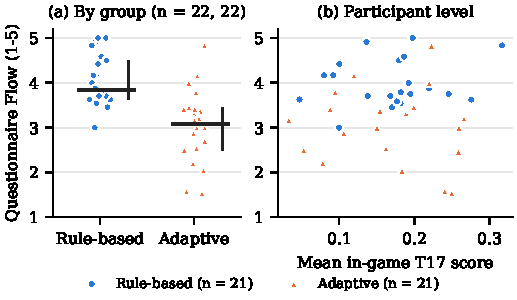
\includegraphics[width=0.6\linewidth]{../figures/FigS1_questionnaire_flow.pdf}
\clearpage\section*{Fig. S2. Telemetry indicators vs.\ questionnaire Flow}Participant level, by condition. (a) Scatter plots with least-squares lines; (b) rank plots (ranks within condition). Used to inspect differences between Pearson $r$ and Spearman $\rho$.\\[4pt]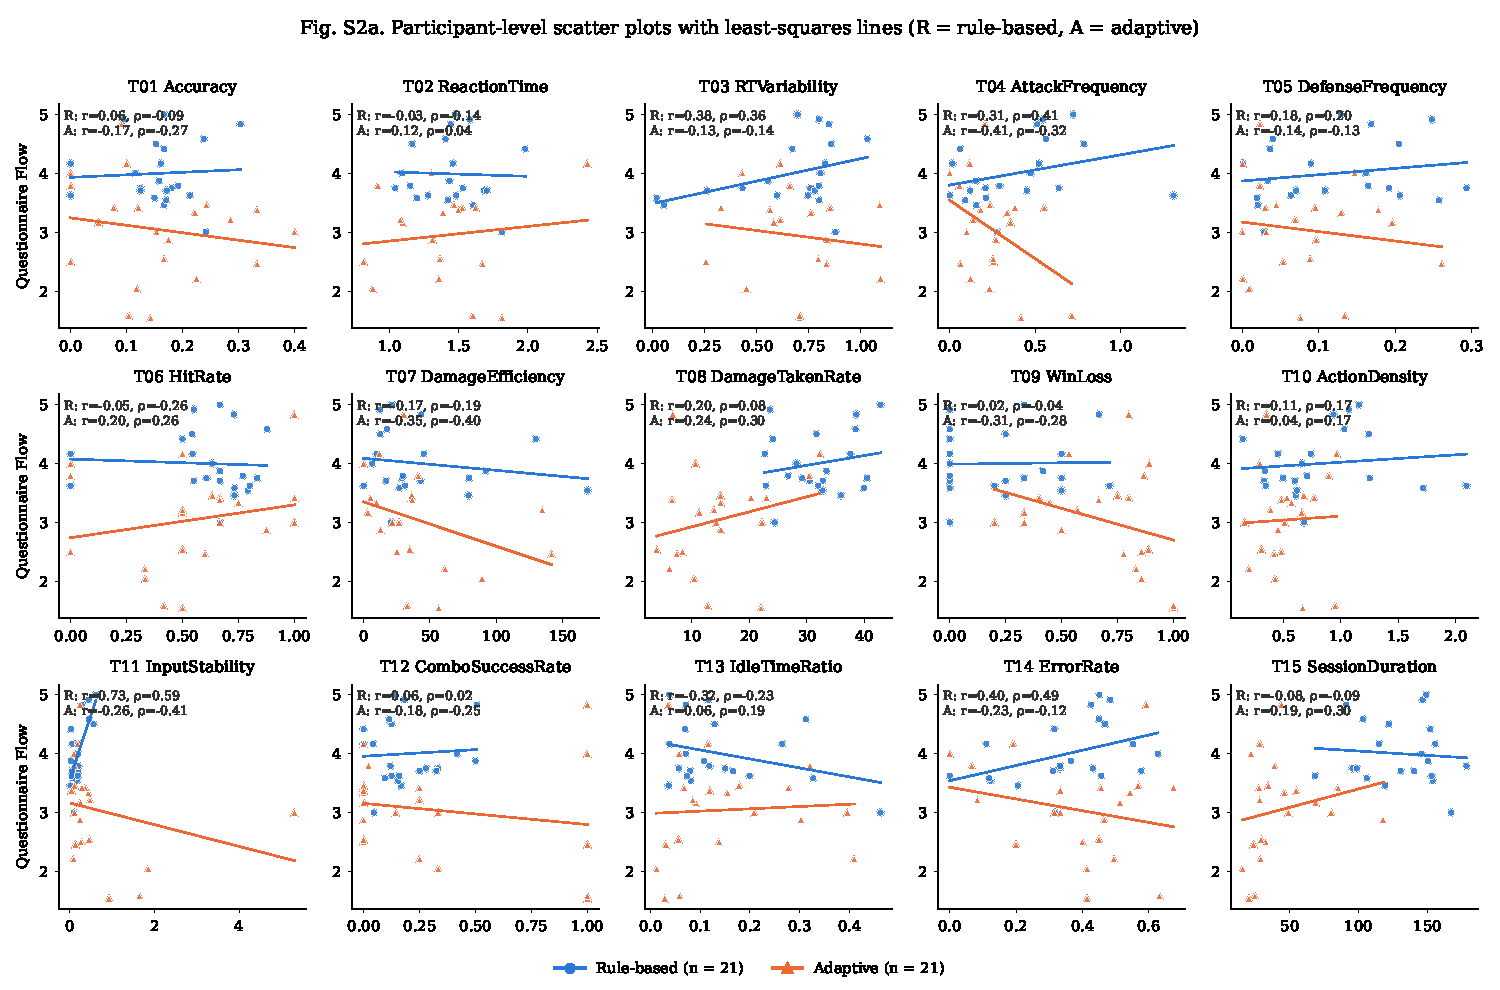
\includegraphics[width=0.92\linewidth]{../figures/FigS2a_scatter_telemetry_vs_flow.pdf}\clearpage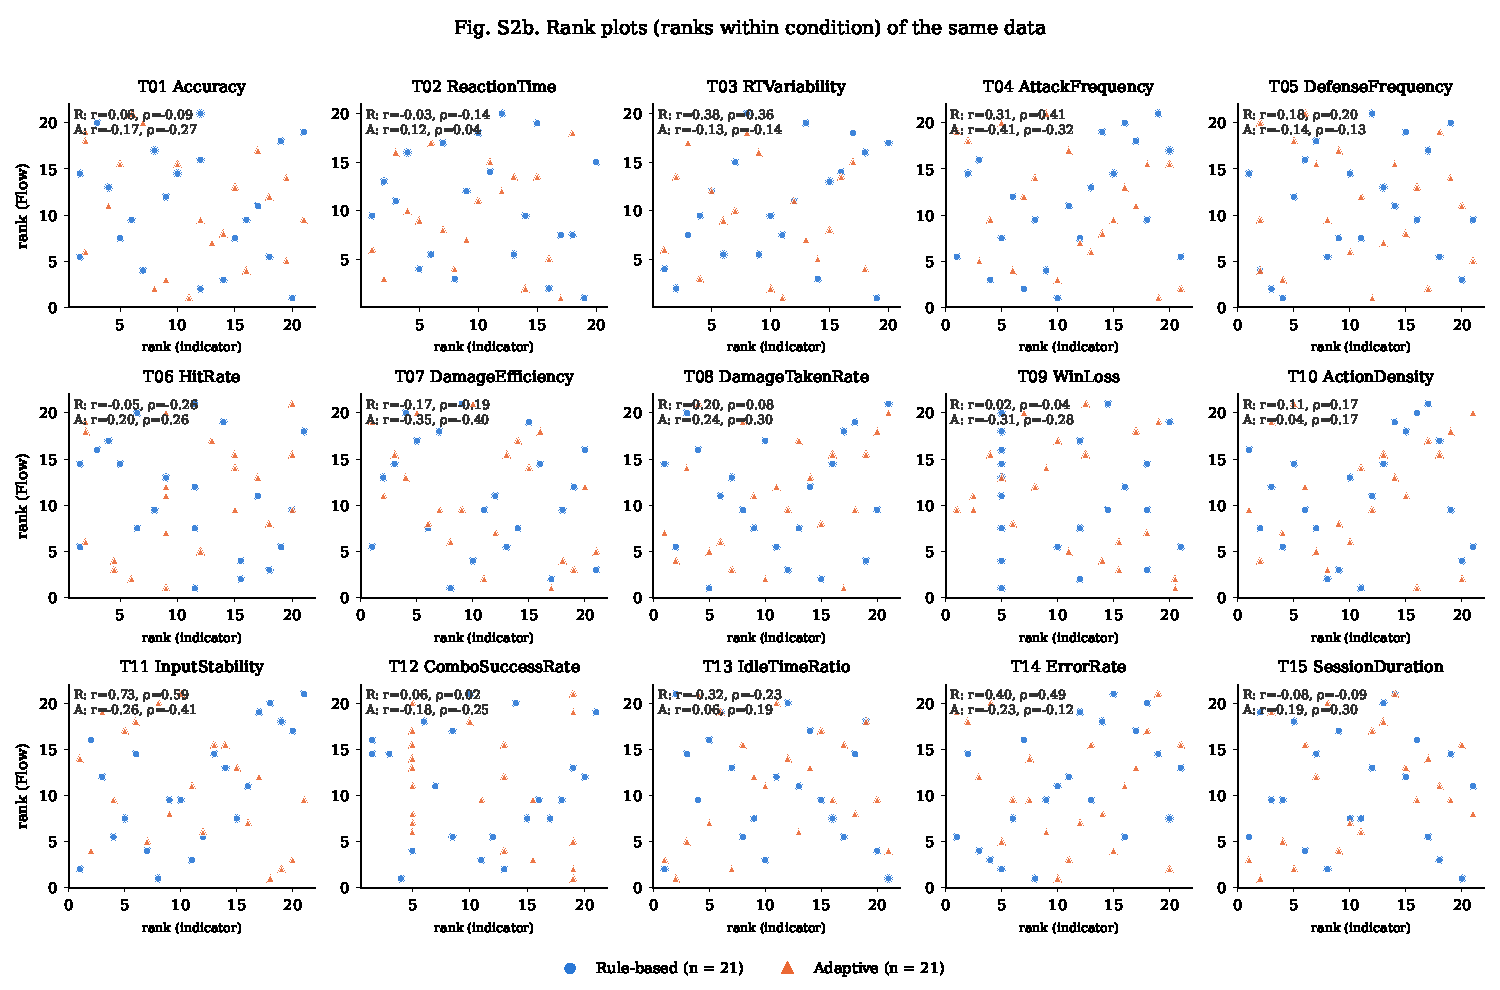
\includegraphics[width=0.92\linewidth]{../figures/FigS2b_rank_telemetry_vs_flow.pdf}
\clearpage\section*{Fig. S3. Distributions}Participant-level histograms of questionnaire Flow (matched participants) and T01--T15 by condition; dashed lines = medians.\\[4pt]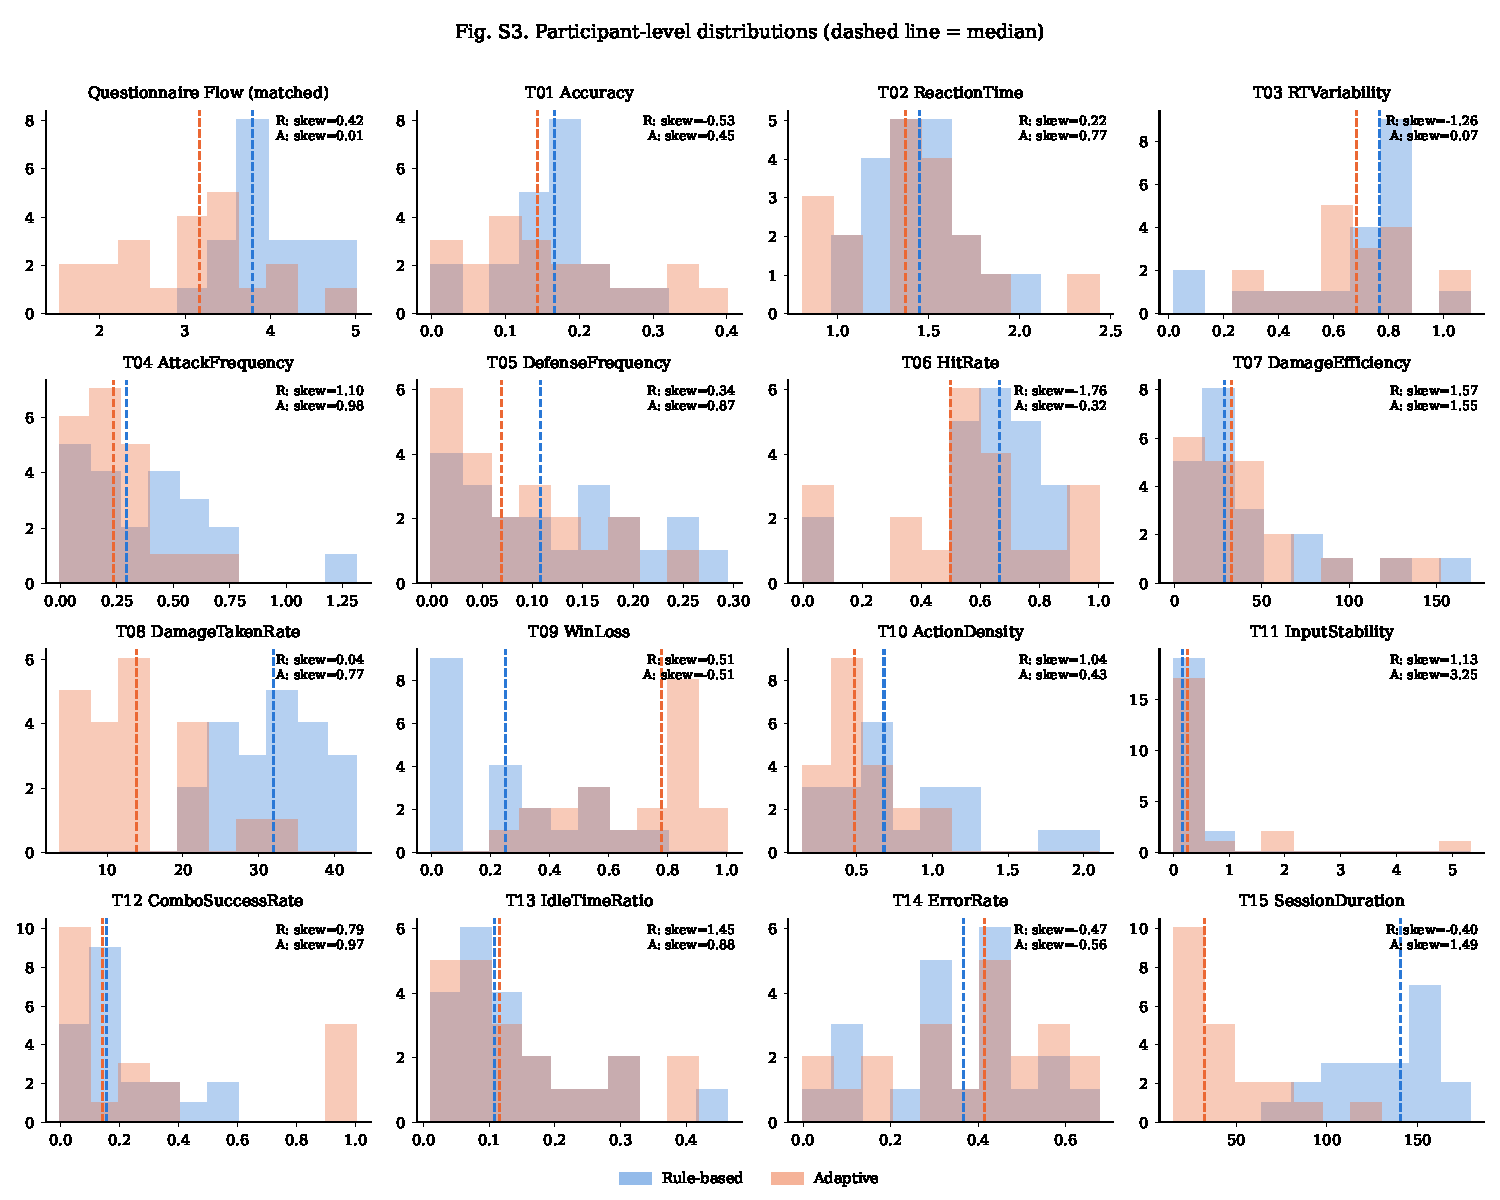
\includegraphics[width=0.85\linewidth]{../figures/FigS3_distributions.pdf}\clearpage
\section*{Table S1. Dataset summary by condition}
Encounter = one boss fight; participant = one tester within one condition.

{\scriptsize\setlength{\tabcolsep}{3pt}\begin{longtable}{lrr}
\toprule
measure & Rule-based & Adaptive \\
\midrule
\endhead
participants\_telemetry & 24.000 & 21.000 \\
questionnaire\_responses & 22.000 & 22.000 \\
participants\_matched & 21.000 & 21.000 \\
encounters & 113.000 & 206.000 \\
encounters\_per\_participant\_median & 4.000 & 7.000 \\
min & 2.000 & 2.000 \\
max & 12.000 & 37.000 \\
duration\_median\_s & 130.350 & 29.500 \\
duration\_q1 & 103.490 & 16.860 \\
duration\_q3 & 155.710 & 54.580 \\
wins & 28.000 & 157.000 \\
win\_pct & 24.780 & 76.210 \\
max\_boss\_level & 5.000 & 31.000 \\
T17\_zero & 8.000 & 25.000 \\
reaction\_samples\_lt2 & 40.000 & 133.000 \\
T11\_gt50 & 0.000 & 8.000 \\
\bottomrule
\end{longtable}}

\section*{Table S2. Questionnaire reliability (Cronbach alpha) by scale and condition}
{\scriptsize\setlength{\tabcolsep}{3pt}\begin{longtable}{lrrrrr}
\toprule
condition & scale & alpha & mean & sd & mean\_inter\_item\_r \\
\midrule
\endhead
Rule-based & All 24 items & 0.917 & 4.045 & 0.562 & 0.333 \\
Rule-based & Concentration & 0.781 & 4.148 & 0.591 & 0.474 \\
Rule-based & Challenge-skill balance & 0.585 & 3.875 & 0.797 & 0.267 \\
Rule-based & Control / system response & 0.845 & 3.943 & 0.824 & 0.575 \\
Rule-based & Enjoyment / motivation & 0.842 & 4.432 & 0.573 & 0.575 \\
Rule-based & Time / deep engagement & 0.732 & 4.000 & 0.744 & 0.444 \\
Rule-based & Pressure / flow experience & 0.795 & 3.875 & 0.801 & 0.545 \\
Adaptive & All 24 items & 0.932 & 3.028 & 0.809 & 0.369 \\
Adaptive & Concentration & 0.777 & 3.284 & 0.989 & 0.470 \\
Adaptive & Challenge-skill balance & 0.510 & 3.159 & 0.918 & 0.167 \\
Adaptive & Control / system response & 0.738 & 3.000 & 0.973 & 0.404 \\
Adaptive & Enjoyment / motivation & 0.876 & 3.125 & 1.023 & 0.641 \\
Adaptive & Time / deep engagement & 0.697 & 3.091 & 0.868 & 0.359 \\
Adaptive & Pressure / flow experience & 0.704 & 2.511 & 0.962 & 0.364 \\
\bottomrule
\end{longtable}}

\section*{Table S3. Questionnaire item statistics}
Floor/ceiling = \% of responses at 1/5. Corrected item--total r uses the 24-item total; item--rest r and alpha if deleted use the item's dimension.

{\scriptsize\setlength{\tabcolsep}{3pt}\begin{longtable}{lrrrrrrrrr}
\toprule
condition & dimension & item & mean & sd & floor\_pct & ceiling\_pct & corrected\_item\_total\_r\_scale & item\_rest\_r\_dimension & alpha\_if\_deleted\_dimension \\
\midrule
\endhead
Rule-based & Concentration & q1 & 4.273 & 0.631 & 0.000 & 36.364 & 0.689 & 0.454 & 0.788 \\
Rule-based & Concentration & q2 & 4.182 & 0.733 & 0.000 & 36.364 & 0.422 & 0.657 & 0.692 \\
Rule-based & Concentration & q3 & 3.864 & 0.889 & 0.000 & 22.727 & 0.471 & 0.596 & 0.730 \\
Rule-based & Concentration & q4 & 4.273 & 0.767 & 0.000 & 45.455 & 0.513 & 0.664 & 0.686 \\
Rule-based & Challenge-skill balance & q5 & 3.727 & 1.279 & 0.000 & 40.909 & 0.513 & 0.564 & 0.333 \\
Rule-based & Challenge-skill balance & q6 & 3.909 & 1.306 & 4.545 & 50.000 & 0.525 & 0.150 & 0.688 \\
Rule-based & Challenge-skill balance & q7 & 3.773 & 1.110 & 0.000 & 36.364 & 0.564 & 0.558 & 0.366 \\
Rule-based & Challenge-skill balance & q8 & 4.091 & 1.065 & 0.000 & 50.000 & 0.321 & 0.264 & 0.584 \\
Rule-based & Control / system response & q9 & 3.773 & 1.110 & 0.000 & 36.364 & 0.564 & 0.760 & 0.767 \\
Rule-based & Control / system response & q10 & 3.909 & 1.065 & 0.000 & 36.364 & 0.500 & 0.779 & 0.758 \\
Rule-based & Control / system response & q11 & 4.000 & 0.926 & 0.000 & 36.364 & 0.737 & 0.510 & 0.870 \\
Rule-based & Control / system response & q12 & 4.091 & 0.868 & 0.000 & 36.364 & 0.488 & 0.703 & 0.799 \\
Rule-based & Enjoyment / motivation & q13 & 4.727 & 0.550 & 0.000 & 77.273 & 0.419 & 0.691 & 0.805 \\
Rule-based & Enjoyment / motivation & q14 & 4.409 & 0.666 & 0.000 & 50.000 & 0.522 & 0.454 & 0.888 \\
Rule-based & Enjoyment / motivation & q15 & 4.227 & 0.813 & 0.000 & 40.909 & 0.562 & 0.789 & 0.749 \\
Rule-based & Enjoyment / motivation & q16 & 4.364 & 0.727 & 0.000 & 50.000 & 0.646 & 0.838 & 0.724 \\
Rule-based & Time / deep engagement & q17 & 4.045 & 1.046 & 4.545 & 40.909 & 0.530 & 0.293 & 0.802 \\
Rule-based & Time / deep engagement & q18 & 4.182 & 0.795 & 0.000 & 36.364 & 0.450 & 0.703 & 0.597 \\
Rule-based & Time / deep engagement & q19 & 3.636 & 1.293 & 9.091 & 31.818 & 0.614 & 0.628 & 0.619 \\
Rule-based & Time / deep engagement & q20 & 4.136 & 0.774 & 0.000 & 36.364 & 0.661 & 0.616 & 0.641 \\
Rule-based & Pressure / flow experience & q21 & 4.000 & 1.113 & 4.545 & 40.909 & 0.681 & 0.560 & 0.771 \\
Rule-based & Pressure / flow experience & q22 & 4.273 & 0.631 & 0.000 & 36.364 & 0.582 & 0.615 & 0.772 \\
Rule-based & Pressure / flow experience & q23 & 3.318 & 1.287 & 4.545 & 27.273 & 0.588 & 0.558 & 0.797 \\
Rule-based & Pressure / flow experience & q24 & 3.909 & 0.921 & 0.000 & 31.818 & 0.699 & 0.850 & 0.631 \\
Adaptive & Concentration & q1 & 3.409 & 1.297 & 4.545 & 27.273 & 0.652 & 0.691 & 0.662 \\
Adaptive & Concentration & q2 & 3.500 & 1.336 & 9.091 & 27.273 & 0.801 & 0.732 & 0.636 \\
Adaptive & Concentration & q3 & 3.091 & 1.306 & 9.091 & 18.182 & 0.346 & 0.255 & 0.879 \\
Adaptive & Concentration & q4 & 3.136 & 1.167 & 4.545 & 13.636 & 0.787 & 0.712 & 0.660 \\
Adaptive & Challenge-skill balance & q5 & 3.045 & 1.588 & 22.727 & 31.818 & 0.703 & 0.643 & 0.041 \\
Adaptive & Challenge-skill balance & q6 & 2.591 & 1.623 & 40.909 & 18.182 & 0.337 & 0.434 & 0.297 \\
Adaptive & Challenge-skill balance & q7 & 2.818 & 1.332 & 27.273 & 9.091 & 0.329 & 0.422 & 0.336 \\
Adaptive & Challenge-skill balance & q8 & 4.182 & 1.181 & 4.545 & 54.545 & 0.115 & -0.194 & 0.746 \\
Adaptive & Control / system response & q9 & 2.682 & 1.287 & 13.636 & 13.636 & 0.684 & 0.730 & 0.557 \\
Adaptive & Control / system response & q10 & 2.727 & 1.420 & 18.182 & 18.182 & 0.655 & 0.604 & 0.632 \\
Adaptive & Control / system response & q11 & 3.364 & 1.293 & 9.091 & 27.273 & 0.684 & 0.607 & 0.633 \\
Adaptive & Control / system response & q12 & 3.227 & 1.193 & 9.091 & 13.636 & 0.418 & 0.222 & 0.826 \\
Adaptive & Enjoyment / motivation & q13 & 3.455 & 1.184 & 4.545 & 18.182 & 0.728 & 0.787 & 0.820 \\
Adaptive & Enjoyment / motivation & q14 & 3.409 & 1.054 & 4.545 & 13.636 & 0.764 & 0.672 & 0.866 \\
Adaptive & Enjoyment / motivation & q15 & 2.682 & 1.287 & 18.182 & 13.636 & 0.759 & 0.721 & 0.848 \\
Adaptive & Enjoyment / motivation & q16 & 2.955 & 1.253 & 13.636 & 13.636 & 0.646 & 0.767 & 0.828 \\
Adaptive & Time / deep engagement & q17 & 3.409 & 1.141 & 9.091 & 13.636 & 0.219 & 0.182 & 0.795 \\
Adaptive & Time / deep engagement & q18 & 3.091 & 1.231 & 9.091 & 13.636 & 0.662 & 0.645 & 0.521 \\
Adaptive & Time / deep engagement & q19 & 2.591 & 1.221 & 22.727 & 9.091 & 0.652 & 0.421 & 0.671 \\
Adaptive & Time / deep engagement & q20 & 3.273 & 1.202 & 9.091 & 18.182 & 0.820 & 0.740 & 0.455 \\
Adaptive & Pressure / flow experience & q21 & 2.318 & 1.211 & 36.364 & 4.545 & 0.654 & 0.377 & 0.704 \\
Adaptive & Pressure / flow experience & q22 & 3.318 & 1.211 & 4.545 & 22.727 & 0.330 & 0.349 & 0.718 \\
Adaptive & Pressure / flow experience & q23 & 2.227 & 1.510 & 50.000 & 13.636 & 0.702 & 0.641 & 0.533 \\
Adaptive & Pressure / flow experience & q24 & 2.182 & 1.332 & 40.909 & 9.091 & 0.673 & 0.614 & 0.560 \\
\bottomrule
\end{longtable}}

\section*{Table S4. Descriptive statistics of questionnaire Flow (mean of 24 items)}
Outliers: Tukey rule (beyond 1.5 IQR).

{\scriptsize\setlength{\tabcolsep}{3pt}\begin{longtable}{lrrrrrrrrrrrrr}
\toprule
condition & n & mean & sd & median & q1 & q3 & min & max & skewness & kurtosis\_excess & shapiro\_p & missing\_pct & outliers\_tukey\_n \\
\midrule
\endhead
Rule-based & 22 & 4.045 & 0.562 & 3.833 & 3.646 & 4.479 & 3.000 & 5.000 & 0.365 & -0.842 & 0.103 & 0.000 & 0 \\
Adaptive & 22 & 3.028 & 0.809 & 3.083 & 2.510 & 3.417 & 1.542 & 4.833 & 0.064 & -0.144 & 0.942 & 0.000 & 1 \\
\bottomrule
\end{longtable}}

\section*{Table S5. Descriptive statistics of telemetry indicators T01--T15}
Participant level = median per participant (T09 = win rate); encounter level = all encounters. Missing = undefined values (T02/T03 with fewer than 2 reaction samples).

{\scriptsize\setlength{\tabcolsep}{3pt}\begin{longtable}{lrrrrrrrrrrrrrrrr}
\toprule
condition & level & indicator & unit & n & mean & sd & median & q1 & q3 & min & max & skewness & kurtosis\_excess & shapiro\_p & missing\_pct & outliers\_tukey\_n \\
\midrule
\endhead
Rule-based & participant & T01\_Accuracy & ratio 0-1 & 21 & 0.157 & 0.070 & 0.167 & 0.125 & 0.180 & 0.000 & 0.304 & -0.529 & 0.950 & 0.078 & 0.000 & 3 \\
Rule-based & encounter & T01\_Accuracy & ratio 0-1 & 113 & 0.160 & 0.118 & 0.154 & 0.095 & 0.208 & 0.000 & 0.625 & 1.302 & 2.984 & 0.000 & 0.000 & 5 \\
Rule-based & participant & T02\_ReactionTime & s & 20 & 1.446 & 0.245 & 1.449 & 1.258 & 1.585 & 1.041 & 1.981 & 0.216 & -0.401 & 0.781 & 4.762 & 0 \\
Rule-based & encounter & T02\_ReactionTime & s & 73 & 1.411 & 0.433 & 1.403 & 1.124 & 1.604 & 0.408 & 2.723 & 0.350 & 0.396 & 0.455 & 35.398 & 1 \\
Rule-based & participant & T03\_RTVariability & s & 20 & 0.661 & 0.272 & 0.768 & 0.586 & 0.812 & 0.019 & 1.032 & -1.262 & 0.648 & 0.003 & 4.762 & 2 \\
Rule-based & encounter & T03\_RTVariability & s & 73 & 0.693 & 0.300 & 0.757 & 0.553 & 0.881 & 0.019 & 1.359 & -0.615 & 0.215 & 0.000 & 35.398 & 4 \\
Rule-based & participant & T04\_AttackFrequency & attacks/s & 21 & 0.386 & 0.318 & 0.291 & 0.152 & 0.543 & 0.000 & 1.308 & 1.102 & 1.303 & 0.040 & 0.000 & 1 \\
Rule-based & encounter & T04\_AttackFrequency & attacks/s & 113 & 0.450 & 0.476 & 0.322 & 0.125 & 0.654 & 0.000 & 3.137 & 2.297 & 8.312 & 0.000 & 0.000 & 4 \\
Rule-based & participant & T05\_DefenseFrequency & actions/s & 21 & 0.120 & 0.090 & 0.108 & 0.036 & 0.192 & 0.000 & 0.293 & 0.343 & -1.153 & 0.127 & 0.000 & 0 \\
Rule-based & encounter & T05\_DefenseFrequency & actions/s & 113 & 0.510 & 4.224 & 0.083 & 0.028 & 0.180 & 0.000 & 45.000 & 10.478 & 107.867 & 0.000 & 0.000 & 3 \\
Rule-based & participant & T06\_HitRate & ratio 0-1 & 21 & 0.612 & 0.229 & 0.667 & 0.550 & 0.732 & 0.000 & 0.878 & -1.760 & 2.618 & 0.000 & 0.000 & 2 \\
Rule-based & encounter & T06\_HitRate & ratio 0-1 & 113 & 0.599 & 0.283 & 0.667 & 0.524 & 0.750 & 0.000 & 1.000 & -1.034 & 0.305 & 0.000 & 0.000 & 16 \\
Rule-based & participant & T07\_DamageEfficiency & damage/attack & 21 & 43.601 & 43.364 & 28.934 & 16.975 & 45.276 & 0.000 & 168.818 & 1.574 & 1.754 & 0.001 & 0.000 & 3 \\
Rule-based & encounter & T07\_DamageEfficiency & damage/attack & 113 & 104.020 & 332.850 & 22.208 & 9.766 & 66.723 & 0.000 & 2400 & 5.601 & 31.670 & 0.000 & 0.000 & 13 \\
Rule-based & participant & T08\_DamageTakenRate & damage/s & 21 & 31.823 & 6.327 & 31.974 & 26.739 & 37.566 & 22.653 & 42.786 & 0.044 & -1.181 & 0.281 & 0.000 & 0 \\
Rule-based & encounter & T08\_DamageTakenRate & damage/s & 113 & 67.217 & 363.940 & 31.974 & 25.799 & 39.202 & 0.000 & 3900 & 10.474 & 107.811 & 0.000 & 0.000 & 4 \\
Rule-based & participant & T09\_WinLoss & win rate (0-1) & 21 & 0.234 & 0.243 & 0.250 & 0.000 & 0.417 & 0.000 & 0.714 & 0.505 & -1.009 & 0.004 & 0.000 & 0 \\
Rule-based & encounter & T09\_WinLoss & win rate (0-1) & 113 & 0.239 & 0.428 & 0.000 & 0.000 & 0.000 & 0.000 & 1.000 & 1.224 & -0.501 & 0.000 & 0.000 & 27 \\
Rule-based & participant & T10\_ActionDensity & actions/s & 21 & 0.821 & 0.481 & 0.680 & 0.497 & 1.070 & 0.145 & 2.096 & 1.040 & 0.719 & 0.069 & 0.000 & 1 \\
Rule-based & encounter & T10\_ActionDensity & actions/s & 113 & 1.423 & 5.609 & 0.679 & 0.443 & 1.186 & 0.000 & 60.000 & 10.214 & 104.164 & 0.000 & 0.000 & 8 \\
Rule-based & participant & T11\_InputStability & 1/variance (s\textasciicircum{}-2) & 21 & 0.195 & 0.177 & 0.161 & 0.055 & 0.200 & 0.015 & 0.613 & 1.132 & 0.198 & 0.003 & 0.000 & 4 \\
Rule-based & encounter & T11\_InputStability & 1/variance (s\textasciicircum{}-2) & 113 & 0.290 & 0.391 & 0.127 & 0.041 & 0.420 & 0.000 & 2.201 & 2.217 & 5.770 & 0.000 & 0.000 & 9 \\
Rule-based & participant & T12\_ComboSuccessRate & ratio 0-1 & 21 & 0.194 & 0.149 & 0.155 & 0.114 & 0.278 & 0.000 & 0.505 & 0.791 & -0.309 & 0.049 & 0.000 & 0 \\
Rule-based & encounter & T12\_ComboSuccessRate & ratio 0-1 & 113 & 0.239 & 0.252 & 0.146 & 0.053 & 0.333 & 0.000 & 1.000 & 1.341 & 1.293 & 0.000 & 0.000 & 5 \\
Rule-based & participant & T13\_IdleTimeRatio & ratio 0-1 & 21 & 0.141 & 0.113 & 0.108 & 0.071 & 0.166 & 0.037 & 0.462 & 1.448 & 1.336 & 0.001 & 0.000 & 3 \\
Rule-based & encounter & T13\_IdleTimeRatio & ratio 0-1 & 113 & 0.165 & 0.166 & 0.117 & 0.070 & 0.204 & 0.003 & 1.000 & 2.728 & 9.784 & 0.000 & 0.000 & 9 \\
Rule-based & participant & T14\_ErrorRate & ratio 0-1 & 21 & 0.355 & 0.167 & 0.366 & 0.312 & 0.457 & 0.000 & 0.627 & -0.474 & -0.532 & 0.371 & 0.000 & 1 \\
Rule-based & encounter & T14\_ErrorRate & ratio 0-1 & 113 & 0.362 & 0.212 & 0.373 & 0.216 & 0.514 & 0.000 & 0.830 & -0.103 & -0.698 & 0.010 & 0.000 & 0 \\
Rule-based & participant & T15\_SessionDuration & s & 21 & 130.725 & 28.803 & 140.340 & 106.090 & 152.210 & 68.490 & 178.590 & -0.402 & -0.738 & 0.376 & 0.000 & 0 \\
Rule-based & encounter & T15\_SessionDuration & s & 113 & 130.196 & 48.432 & 130.350 & 103.490 & 155.710 & 1.000 & 419.960 & 1.728 & 10.138 & 0.000 & 0.000 & 3 \\
Adaptive & participant & T01\_Accuracy & ratio 0-1 & 21 & 0.159 & 0.114 & 0.143 & 0.091 & 0.225 & 0.000 & 0.400 & 0.448 & -0.598 & 0.395 & 0.000 & 0 \\
Adaptive & encounter & T01\_Accuracy & ratio 0-1 & 206 & 0.166 & 0.198 & 0.116 & 0.000 & 0.250 & 0.000 & 1.000 & 2.013 & 5.541 & 0.000 & 0.000 & 5 \\
Adaptive & participant & T02\_ReactionTime & s & 18 & 1.396 & 0.383 & 1.374 & 1.146 & 1.583 & 0.811 & 2.430 & 0.768 & 1.172 & 0.229 & 14.286 & 1 \\
Adaptive & encounter & T02\_ReactionTime & s & 73 & 1.397 & 0.523 & 1.385 & 1.025 & 1.669 & 0.554 & 2.989 & 0.613 & 0.531 & 0.026 & 64.563 & 2 \\
Adaptive & participant & T03\_RTVariability & s & 18 & 0.676 & 0.229 & 0.682 & 0.568 & 0.824 & 0.256 & 1.094 & 0.075 & -0.392 & 0.822 & 14.286 & 0 \\
Adaptive & encounter & T03\_RTVariability & s & 73 & 0.612 & 0.334 & 0.681 & 0.317 & 0.869 & 0.007 & 1.415 & 0.050 & -0.928 & 0.037 & 64.563 & 0 \\
Adaptive & participant & T04\_AttackFrequency & attacks/s & 21 & 0.252 & 0.171 & 0.235 & 0.122 & 0.336 & 0.000 & 0.714 & 0.977 & 0.898 & 0.176 & 0.000 & 1 \\
Adaptive & encounter & T04\_AttackFrequency & attacks/s & 206 & 0.280 & 0.320 & 0.197 & 0.030 & 0.381 & 0.000 & 1.880 & 1.765 & 4.017 & 0.000 & 0.000 & 12 \\
Adaptive & participant & T05\_DefenseFrequency & actions/s & 21 & 0.080 & 0.072 & 0.069 & 0.023 & 0.129 & 0.000 & 0.260 & 0.869 & 0.016 & 0.062 & 0.000 & 0 \\
Adaptive & encounter & T05\_DefenseFrequency & actions/s & 206 & 0.092 & 0.102 & 0.063 & 0.000 & 0.145 & 0.000 & 0.607 & 1.471 & 2.906 & 0.000 & 0.000 & 4 \\
Adaptive & participant & T06\_HitRate & ratio 0-1 & 21 & 0.545 & 0.303 & 0.500 & 0.417 & 0.667 & 0.000 & 1.000 & -0.319 & -0.431 & 0.114 & 0.000 & 3 \\
Adaptive & encounter & T06\_HitRate & ratio 0-1 & 206 & 0.468 & 0.400 & 0.500 & 0.000 & 0.800 & 0.000 & 1.000 & 0.034 & -1.523 & 0.000 & 0.000 & 0 \\
Adaptive & participant & T07\_DamageEfficiency & damage/attack & 21 & 40.414 & 38.755 & 32.944 & 12.795 & 41.201 & 0.000 & 141.750 & 1.551 & 1.632 & 0.001 & 0.000 & 3 \\
Adaptive & encounter & T07\_DamageEfficiency & damage/attack & 206 & 116.594 & 381.693 & 30.673 & 0.646 & 92.092 & 0.000 & 4123 & 8.238 & 76.023 & 0.000 & 0.000 & 19 \\
Adaptive & participant & T08\_DamageTakenRate & damage/s & 21 & 14.631 & 7.838 & 13.851 & 8.389 & 20.278 & 3.869 & 32.213 & 0.770 & -0.202 & 0.107 & 0.000 & 0 \\
Adaptive & encounter & T08\_DamageTakenRate & damage/s & 206 & 21.769 & 22.404 & 15.258 & 5.895 & 31.483 & 0.000 & 144.912 & 1.907 & 5.184 & 0.000 & 0.000 & 9 \\
Adaptive & participant & T09\_WinLoss & win rate (0-1) & 21 & 0.681 & 0.238 & 0.778 & 0.500 & 0.857 & 0.200 & 1.000 & -0.509 & -0.977 & 0.086 & 0.000 & 0 \\
Adaptive & encounter & T09\_WinLoss & win rate (0-1) & 206 & 0.767 & 0.424 & 1.000 & 1.000 & 1.000 & 0.000 & 1.000 & -1.263 & -0.405 & 0.000 & 0.000 & 48 \\
Adaptive & participant & T10\_ActionDensity & actions/s & 21 & 0.532 & 0.229 & 0.483 & 0.390 & 0.669 & 0.161 & 0.964 & 0.426 & -0.598 & 0.454 & 0.000 & 0 \\
Adaptive & encounter & T10\_ActionDensity & actions/s & 206 & 0.613 & 0.463 & 0.483 & 0.275 & 0.890 & 0.012 & 2.572 & 1.221 & 1.510 & 0.000 & 0.000 & 4 \\
Adaptive & participant & T11\_InputStability & 1/variance (s\textasciicircum{}-2) & 21 & 0.646 & 1.174 & 0.245 & 0.113 & 0.453 & 0.036 & 5.308 & 3.248 & 10.183 & 0.000 & 0.000 & 3 \\
Adaptive & encounter & T11\_InputStability & 1/variance (s\textasciicircum{}-2) & 206 & 24.450 & 172.780 & 0.209 & 0.035 & 1.151 & 0.000 & 1953 & 9.300 & 91.536 & 0.000 & 0.000 & 35 \\
Adaptive & participant & T12\_ComboSuccessRate & ratio 0-1 & 21 & 0.313 & 0.410 & 0.143 & 0.000 & 0.333 & 0.000 & 1.000 & 0.972 & -0.767 & 0.000 & 0.000 & 5 \\
Adaptive & encounter & T12\_ComboSuccessRate & ratio 0-1 & 206 & 0.401 & 0.445 & 0.174 & 0.000 & 1.000 & 0.000 & 1.000 & 0.468 & -1.597 & 0.000 & 0.000 & 0 \\
Adaptive & participant & T13\_IdleTimeRatio & ratio 0-1 & 21 & 0.150 & 0.123 & 0.116 & 0.058 & 0.209 & 0.013 & 0.409 & 0.884 & -0.470 & 0.011 & 0.000 & 0 \\
Adaptive & encounter & T13\_IdleTimeRatio & ratio 0-1 & 206 & 0.154 & 0.175 & 0.091 & 0.029 & 0.229 & 0.000 & 0.953 & 1.652 & 2.756 & 0.000 & 0.000 & 9 \\
Adaptive & participant & T14\_ErrorRate & ratio 0-1 & 21 & 0.388 & 0.189 & 0.414 & 0.316 & 0.513 & 0.000 & 0.674 & -0.560 & -0.586 & 0.315 & 0.000 & 1 \\
Adaptive & encounter & T14\_ErrorRate & ratio 0-1 & 206 & 0.322 & 0.249 & 0.333 & 0.041 & 0.510 & 0.000 & 0.875 & 0.082 & -1.193 & 0.000 & 0.000 & 0 \\
Adaptive & participant & T15\_SessionDuration & s & 21 & 42.910 & 25.782 & 32.410 & 27.830 & 49.130 & 15.845 & 117.895 & 1.491 & 1.602 & 0.002 & 0.000 & 2 \\
Adaptive & encounter & T15\_SessionDuration & s & 206 & 49.837 & 77.088 & 29.505 & 16.863 & 54.583 & 3.660 & 899.800 & 7.197 & 71.304 & 0.000 & 0.000 & 19 \\
\bottomrule
\end{longtable}}

\section*{Table S6. Correlations of telemetry indicators with questionnaire Flow (step 3A)}
Participant level, within condition. 95\% CI by Fisher z (Bonett--Wright SE for Spearman). q = Benjamini--Hochberg FDR within each family of 15 tests (condition x method); T17 not included.

{\scriptsize\setlength{\tabcolsep}{3pt}\begin{longtable}{lrrrrrrrrrrrr}
\toprule
condition & indicator & n & pearson\_r & pearson\_ci\_low & pearson\_ci\_high & pearson\_p & spearman\_rho & spearman\_ci\_low & spearman\_ci\_high & spearman\_p & pearson\_q\_BH & spearman\_q\_BH \\
\midrule
\endhead
Rule-based & T01\_Accuracy & 21 & 0.057 & -0.385 & 0.477 & 0.808 & -0.086 & -0.500 & 0.360 & 0.711 & 0.925 & 0.835 \\
Rule-based & T02\_ReactionTime & 20 & -0.034 & -0.469 & 0.415 & 0.888 & -0.138 & -0.549 & 0.327 & 0.562 & 0.925 & 0.835 \\
Rule-based & T03\_RTVariability & 20 & 0.381 & -0.074 & 0.705 & 0.098 & 0.364 & -0.109 & 0.702 & 0.115 & 0.488 & 0.432 \\
Rule-based & T04\_AttackFrequency & 21 & 0.307 & -0.144 & 0.652 & 0.176 & 0.408 & -0.047 & 0.723 & 0.066 & 0.527 & 0.331 \\
Rule-based & T05\_DefenseFrequency & 21 & 0.181 & -0.272 & 0.568 & 0.432 & 0.198 & -0.260 & 0.583 & 0.390 & 0.878 & 0.762 \\
Rule-based & T06\_HitRate & 21 & -0.053 & -0.474 & 0.388 & 0.820 & -0.262 & -0.628 & 0.198 & 0.250 & 0.925 & 0.751 \\
Rule-based & T07\_DamageEfficiency & 21 & -0.167 & -0.559 & 0.285 & 0.468 & -0.191 & -0.578 & 0.266 & 0.407 & 0.878 & 0.762 \\
Rule-based & T08\_DamageTakenRate & 21 & 0.197 & -0.256 & 0.579 & 0.392 & 0.082 & -0.363 & 0.497 & 0.724 & 0.878 & 0.835 \\
Rule-based & T09\_WinLoss & 21 & 0.022 & -0.414 & 0.449 & 0.925 & -0.037 & -0.461 & 0.401 & 0.873 & 0.925 & 0.936 \\
Rule-based & T10\_ActionDensity & 21 & 0.113 & -0.335 & 0.520 & 0.624 & 0.168 & -0.287 & 0.562 & 0.466 & 0.925 & 0.776 \\
Rule-based & T11\_InputStability & 21 & 0.725 & 0.427 & 0.881 & 0.000 & 0.593 & 0.179 & 0.828 & 0.005 & 0.003 & 0.069 \\
Rule-based & T12\_ComboSuccessRate & 21 & 0.063 & -0.379 & 0.482 & 0.785 & 0.016 & -0.418 & 0.445 & 0.944 & 0.925 & 0.944 \\
Rule-based & T13\_IdleTimeRatio & 21 & -0.324 & -0.663 & 0.126 & 0.152 & -0.229 & -0.605 & 0.231 & 0.318 & 0.527 & 0.762 \\
Rule-based & T14\_ErrorRate & 21 & 0.405 & -0.032 & 0.712 & 0.069 & 0.486 & 0.043 & 0.770 & 0.025 & 0.488 & 0.190 \\
Rule-based & T15\_SessionDuration & 21 & -0.079 & -0.494 & 0.365 & 0.733 & -0.090 & -0.503 & 0.357 & 0.699 & 0.925 & 0.835 \\
Rule-based & T17\_mean & 21 & 0.175 & -0.278 & 0.564 & 0.448 & 0.181 & -0.276 & 0.571 & 0.433 &  &  \\
Adaptive & T01\_Accuracy & 21 & -0.174 & -0.563 & 0.279 & 0.450 & -0.270 & -0.634 & 0.191 & 0.236 & 0.676 & 0.454 \\
Adaptive & T02\_ReactionTime & 18 & 0.123 & -0.365 & 0.558 & 0.628 & 0.040 & -0.435 & 0.498 & 0.874 & 0.724 & 0.874 \\
Adaptive & T03\_RTVariability & 18 & -0.135 & -0.566 & 0.355 & 0.594 & -0.144 & -0.574 & 0.349 & 0.570 & 0.724 & 0.658 \\
Adaptive & T04\_AttackFrequency & 21 & -0.410 & -0.715 & 0.026 & 0.065 & -0.319 & -0.666 & 0.142 & 0.159 & 0.676 & 0.454 \\
Adaptive & T05\_DefenseFrequency & 21 & -0.140 & -0.539 & 0.310 & 0.545 & -0.132 & -0.535 & 0.320 & 0.568 & 0.724 & 0.658 \\
Adaptive & T06\_HitRate & 21 & 0.205 & -0.249 & 0.585 & 0.374 & 0.261 & -0.200 & 0.627 & 0.254 & 0.676 & 0.454 \\
Adaptive & T07\_DamageEfficiency & 21 & -0.353 & -0.681 & 0.093 & 0.117 & -0.402 & -0.719 & 0.055 & 0.071 & 0.676 & 0.454 \\
Adaptive & T08\_DamageTakenRate & 21 & 0.242 & -0.212 & 0.610 & 0.290 & 0.302 & -0.159 & 0.655 & 0.183 & 0.676 & 0.454 \\
Adaptive & T09\_WinLoss & 21 & -0.310 & -0.654 & 0.140 & 0.171 & -0.276 & -0.637 & 0.185 & 0.226 & 0.676 & 0.454 \\
Adaptive & T10\_ActionDensity & 21 & 0.038 & -0.400 & 0.462 & 0.870 & 0.172 & -0.284 & 0.564 & 0.457 & 0.870 & 0.623 \\
Adaptive & T11\_InputStability & 21 & -0.262 & -0.623 & 0.191 & 0.251 & -0.411 & -0.725 & 0.045 & 0.064 & 0.676 & 0.454 \\
Adaptive & T12\_ComboSuccessRate & 21 & -0.179 & -0.567 & 0.274 & 0.437 & -0.251 & -0.620 & 0.210 & 0.273 & 0.676 & 0.454 \\
Adaptive & T13\_IdleTimeRatio & 21 & 0.059 & -0.383 & 0.478 & 0.800 & 0.190 & -0.267 & 0.578 & 0.408 & 0.857 & 0.613 \\
Adaptive & T14\_ErrorRate & 21 & -0.228 & -0.601 & 0.226 & 0.320 & -0.117 & -0.523 & 0.333 & 0.615 & 0.676 & 0.658 \\
Adaptive & T15\_SessionDuration & 21 & 0.195 & -0.258 & 0.578 & 0.397 & 0.303 & -0.158 & 0.656 & 0.181 & 0.676 & 0.454 \\
Adaptive & T17\_mean & 21 & -0.097 & -0.508 & 0.349 & 0.675 & -0.072 & -0.489 & 0.372 & 0.756 &  &  \\
\bottomrule
\end{longtable}}

\section*{Table S7. Spearman correlation matrix among T01--T15 (rule-based)}
Pearson matrices are provided as CSV files in results/.

{\scriptsize\setlength{\tabcolsep}{3pt}\begin{longtable}{lrrrrrrrrrrrrrrr}
\toprule
 & T01 & T02 & T03 & T04 & T05 & T06 & T07 & T08 & T09 & T10 & T11 & T12 & T13 & T14 & T15 \\
\midrule
\endhead
T01 & 1.000 & 0.245 & 0.185 & 0.322 & -0.157 & 0.656 & 0.301 & 0.464 & 0.155 & 0.293 & 0.159 & 0.022 & 0.142 & 0.020 & -0.226 \\
T02 & 0.245 & 1.000 & -0.117 & -0.084 & -0.317 & -0.063 & 0.165 & -0.018 & -0.095 & -0.200 & -0.295 & -0.114 & -0.194 & -0.035 & 0.095 \\
T03 & 0.185 & -0.117 & 1.000 & 0.287 & 0.323 & 0.008 & -0.376 & -0.257 & -0.142 & 0.202 & 0.568 & -0.209 & 0.147 & 0.322 & 0.239 \\
T04 & 0.322 & -0.084 & 0.287 & 1.000 & 0.122 & 0.397 & -0.438 & 0.449 & -0.016 & 0.842 & 0.783 & 0.147 & 0.257 & 0.790 & -0.530 \\
T05 & -0.157 & -0.317 & 0.323 & 0.122 & 1.000 & -0.011 & -0.091 & -0.191 & 0.307 & 0.114 & 0.374 & 0.383 & -0.304 & 0.087 & 0.056 \\
T06 & 0.656 & -0.063 & 0.008 & 0.397 & -0.011 & 1.000 & 0.217 & 0.591 & 0.137 & 0.515 & 0.224 & 0.224 & 0.187 & 0.101 & -0.348 \\
T07 & 0.301 & 0.165 & -0.376 & -0.438 & -0.091 & 0.217 & 1.000 & 0.100 & 0.567 & -0.366 & -0.475 & 0.125 & -0.313 & -0.506 & 0.027 \\
T08 & 0.464 & -0.018 & -0.257 & 0.449 & -0.191 & 0.591 & 0.100 & 1.000 & 0.207 & 0.482 & 0.225 & 0.257 & -0.021 & 0.175 & -0.590 \\
T09 & 0.155 & -0.095 & -0.142 & -0.016 & 0.307 & 0.137 & 0.567 & 0.207 & 1.000 & 0.015 & -0.097 & 0.403 & -0.372 & -0.227 & -0.285 \\
T10 & 0.293 & -0.200 & 0.202 & 0.842 & 0.114 & 0.515 & -0.366 & 0.482 & 0.015 & 1.000 & 0.638 & -0.057 & 0.303 & 0.429 & -0.474 \\
T11 & 0.159 & -0.295 & 0.568 & 0.783 & 0.374 & 0.224 & -0.475 & 0.225 & -0.097 & 0.638 & 1.000 & 0.081 & 0.229 & 0.700 & -0.192 \\
T12 & 0.022 & -0.114 & -0.209 & 0.147 & 0.383 & 0.224 & 0.125 & 0.257 & 0.403 & -0.057 & 0.081 & 1.000 & -0.231 & 0.298 & -0.391 \\
T13 & 0.142 & -0.194 & 0.147 & 0.257 & -0.304 & 0.187 & -0.313 & -0.021 & -0.372 & 0.303 & 0.229 & -0.231 & 1.000 & 0.229 & -0.170 \\
T14 & 0.020 & -0.035 & 0.322 & 0.790 & 0.087 & 0.101 & -0.506 & 0.175 & -0.227 & 0.429 & 0.700 & 0.298 & 0.229 & 1.000 & -0.335 \\
T15 & -0.226 & 0.095 & 0.239 & -0.530 & 0.056 & -0.348 & 0.027 & -0.590 & -0.285 & -0.474 & -0.192 & -0.391 & -0.170 & -0.335 & 1.000 \\
\bottomrule
\end{longtable}}

\section*{Table S7. Spearman correlation matrix among T01--T15 (adaptive)}
Pearson matrices are provided as CSV files in results/.

{\scriptsize\setlength{\tabcolsep}{3pt}\begin{longtable}{lrrrrrrrrrrrrrrr}
\toprule
 & T01 & T02 & T03 & T04 & T05 & T06 & T07 & T08 & T09 & T10 & T11 & T12 & T13 & T14 & T15 \\
\midrule
\endhead
T01 & 1.000 & 0.297 & 0.443 & -0.163 & 0.070 & 0.471 & 0.385 & -0.225 & -0.374 & -0.363 & 0.030 & -0.036 & 0.205 & -0.000 & 0.194 \\
T02 & 0.297 & 1.000 & 0.375 & 0.267 & 0.131 & 0.504 & 0.005 & 0.309 & -0.030 & 0.424 & -0.007 & 0.138 & -0.203 & 0.197 & -0.172 \\
T03 & 0.443 & 0.375 & 1.000 & 0.086 & -0.179 & 0.297 & 0.333 & 0.053 & 0.036 & 0.044 & -0.158 & 0.079 & 0.166 & 0.294 & -0.015 \\
T04 & -0.163 & 0.267 & 0.086 & 1.000 & 0.248 & 0.259 & -0.204 & 0.240 & -0.051 & 0.474 & 0.412 & -0.181 & -0.118 & 0.694 & 0.116 \\
T05 & 0.070 & 0.131 & -0.179 & 0.248 & 1.000 & 0.049 & -0.194 & -0.257 & 0.007 & 0.052 & -0.099 & -0.074 & -0.295 & 0.118 & 0.057 \\
T06 & 0.471 & 0.504 & 0.297 & 0.259 & 0.049 & 1.000 & -0.249 & 0.178 & -0.665 & -0.071 & 0.105 & -0.158 & 0.213 & 0.394 & 0.624 \\
T07 & 0.385 & 0.005 & 0.333 & -0.204 & -0.194 & -0.249 & 1.000 & -0.238 & 0.388 & -0.095 & 0.025 & 0.367 & -0.270 & -0.205 & -0.504 \\
T08 & -0.225 & 0.309 & 0.053 & 0.240 & -0.257 & 0.178 & -0.238 & 1.000 & -0.285 & 0.674 & 0.088 & -0.145 & 0.290 & -0.121 & 0.121 \\
T09 & -0.374 & -0.030 & 0.036 & -0.051 & 0.007 & -0.665 & 0.388 & -0.285 & 1.000 & 0.016 & 0.095 & 0.463 & -0.509 & -0.087 & -0.727 \\
T10 & -0.363 & 0.424 & 0.044 & 0.474 & 0.052 & -0.071 & -0.095 & 0.674 & 0.016 & 1.000 & 0.005 & -0.276 & 0.010 & 0.186 & -0.039 \\
T11 & 0.030 & -0.007 & -0.158 & 0.412 & -0.099 & 0.105 & 0.025 & 0.088 & 0.095 & 0.005 & 1.000 & 0.208 & -0.318 & 0.215 & -0.171 \\
T12 & -0.036 & 0.138 & 0.079 & -0.181 & -0.074 & -0.158 & 0.367 & -0.145 & 0.463 & -0.276 & 0.208 & 1.000 & -0.495 & -0.184 & -0.610 \\
T13 & 0.205 & -0.203 & 0.166 & -0.118 & -0.295 & 0.213 & -0.270 & 0.290 & -0.509 & 0.010 & -0.318 & -0.495 & 1.000 & 0.051 & 0.703 \\
T14 & -0.000 & 0.197 & 0.294 & 0.694 & 0.118 & 0.394 & -0.205 & -0.121 & -0.087 & 0.186 & 0.215 & -0.184 & 0.051 & 1.000 & 0.292 \\
T15 & 0.194 & -0.172 & -0.015 & 0.116 & 0.057 & 0.624 & -0.504 & 0.121 & -0.727 & -0.039 & -0.171 & -0.610 & 0.703 & 0.292 & 1.000 \\
\bottomrule
\end{longtable}}

\section*{Table S8. Variance inflation factors (complete cases)}
{\scriptsize\setlength{\tabcolsep}{3pt}\begin{longtable}{lrrr}
\toprule
condition & indicator & VIF & n\_complete \\
\midrule
\endhead
Rule-based & T01\_Accuracy & 7.203 & 20 \\
Rule-based & T02\_ReactionTime & 2.429 & 20 \\
Rule-based & T03\_RTVariability & 3.837 & 20 \\
Rule-based & T04\_AttackFrequency & 27.591 & 20 \\
Rule-based & T05\_DefenseFrequency & 3.671 & 20 \\
Rule-based & T06\_HitRate & 19.904 & 20 \\
Rule-based & T07\_DamageEfficiency & 6.466 & 20 \\
Rule-based & T08\_DamageTakenRate & 6.849 & 20 \\
Rule-based & T09\_WinLoss & 7.540 & 20 \\
Rule-based & T10\_ActionDensity & 12.558 & 20 \\
Rule-based & T11\_InputStability & 5.147 & 20 \\
Rule-based & T12\_ComboSuccessRate & 6.070 & 20 \\
Rule-based & T13\_IdleTimeRatio & 4.353 & 20 \\
Rule-based & T14\_ErrorRate & 13.942 & 20 \\
Rule-based & T15\_SessionDuration & 3.707 & 20 \\
Adaptive & T01\_Accuracy & 13.503 & 18 \\
Adaptive & T02\_ReactionTime & 6.959 & 18 \\
Adaptive & T03\_RTVariability & 2.785 & 18 \\
Adaptive & T04\_AttackFrequency & 9.727 & 18 \\
Adaptive & T05\_DefenseFrequency & 13.976 & 18 \\
Adaptive & T06\_HitRate & 41.414 & 18 \\
Adaptive & T07\_DamageEfficiency & 4.898 & 18 \\
Adaptive & T08\_DamageTakenRate & 32.659 & 18 \\
Adaptive & T09\_WinLoss & 4.714 & 18 \\
Adaptive & T10\_ActionDensity & 23.666 & 18 \\
Adaptive & T11\_InputStability & 5.851 & 18 \\
Adaptive & T12\_ComboSuccessRate & 13.414 & 18 \\
Adaptive & T13\_IdleTimeRatio & 7.542 & 18 \\
Adaptive & T14\_ErrorRate & 12.956 & 18 \\
Adaptive & T15\_SessionDuration & 10.390 & 18 \\
\bottomrule
\end{longtable}}

\section*{Table S9. Multiple linear regression of Flow on T01--T15: model fit (step 3B)}
Standardized variables, complete cases. With 4 and 2 residual degrees of freedom the models are overfitted and are reported for completeness only.

{\scriptsize\setlength{\tabcolsep}{3pt}\begin{longtable}{lrrrrrrrrr}
\toprule
condition & n\_complete\_cases & predictors & df\_resid & R2 & adj\_R2 & F & model\_p & max\_VIF & condition\_number \\
\midrule
\endhead
Rule-based & 20 & 15 & 4.000 & 0.942 & 0.725 & 4.347 & 0.083 & 27.591 & 235.528 \\
Adaptive & 18 & 15 & 2.000 & 1.000 & 0.998 & 532.473 & 0.002 & 41.414 & 417.333 \\
\bottomrule
\end{longtable}}

\section*{Table S10. Multiple linear regression coefficients (standardized beta)}
Not interpretable because of overfitting and collinearity; see Table S9.

{\scriptsize\setlength{\tabcolsep}{3pt}\begin{longtable}{lrrrrrrrr}
\toprule
condition & indicator & beta\_std & SE & t & p & ci\_low & ci\_high & VIF \\
\midrule
\endhead
Rule-based & T01\_Accuracy & 0.276 & 0.323 & 0.854 & 0.441 & -0.620 & 1.171 & 7.203 \\
Rule-based & T02\_ReactionTime & 0.173 & 0.187 & 0.922 & 0.409 & -0.347 & 0.693 & 2.429 \\
Rule-based & T03\_RTVariability & 0.399 & 0.235 & 1.692 & 0.166 & -0.255 & 1.052 & 3.837 \\
Rule-based & T04\_AttackFrequency & -1.285 & 0.631 & -2.035 & 0.112 & -3.038 & 0.468 & 27.591 \\
Rule-based & T05\_DefenseFrequency & -0.451 & 0.230 & -1.956 & 0.122 & -1.090 & 0.189 & 3.671 \\
Rule-based & T06\_HitRate & -0.417 & 0.536 & -0.778 & 0.480 & -1.906 & 1.072 & 19.904 \\
Rule-based & T07\_DamageEfficiency & 0.194 & 0.306 & 0.635 & 0.560 & -0.655 & 1.043 & 6.466 \\
Rule-based & T08\_DamageTakenRate & -0.329 & 0.315 & -1.047 & 0.354 & -1.203 & 0.544 & 6.849 \\
Rule-based & T09\_WinLoss & -0.221 & 0.330 & -0.670 & 0.539 & -1.138 & 0.695 & 7.540 \\
Rule-based & T10\_ActionDensity & 1.084 & 0.426 & 2.545 & 0.064 & -0.099 & 2.267 & 12.558 \\
Rule-based & T11\_InputStability & 1.082 & 0.273 & 3.967 & 0.017 & 0.325 & 1.839 & 5.147 \\
Rule-based & T12\_ComboSuccessRate & 0.306 & 0.296 & 1.032 & 0.361 & -0.517 & 1.128 & 6.070 \\
Rule-based & T13\_IdleTimeRatio & -0.733 & 0.251 & -2.923 & 0.043 & -1.430 & -0.037 & 4.353 \\
Rule-based & T14\_ErrorRate & 0.295 & 0.449 & 0.657 & 0.547 & -0.951 & 1.541 & 13.942 \\
Rule-based & T15\_SessionDuration & -0.424 & 0.231 & -1.831 & 0.141 & -1.066 & 0.219 & 3.707 \\
Adaptive & T01\_Accuracy & -0.671 & 0.041 & -16.324 & 0.004 & -0.848 & -0.494 & 13.503 \\
Adaptive & T02\_ReactionTime & -0.813 & 0.030 & -27.563 & 0.001 & -0.940 & -0.686 & 6.959 \\
Adaptive & T03\_RTVariability & -0.207 & 0.019 & -11.066 & 0.008 & -0.287 & -0.126 & 2.785 \\
Adaptive & T04\_AttackFrequency & -0.698 & 0.035 & -20.012 & 0.002 & -0.848 & -0.548 & 9.727 \\
Adaptive & T05\_DefenseFrequency & -0.729 & 0.042 & -17.420 & 0.003 & -0.909 & -0.549 & 13.976 \\
Adaptive & T06\_HitRate & 2.432 & 0.072 & 33.782 & 0.001 & 2.123 & 2.742 & 41.414 \\
Adaptive & T07\_DamageEfficiency & -0.771 & 0.025 & -31.147 & 0.001 & -0.878 & -0.665 & 4.898 \\
Adaptive & T08\_DamageTakenRate & -1.473 & 0.064 & -23.036 & 0.002 & -1.748 & -1.198 & 32.659 \\
Adaptive & T09\_WinLoss & -0.332 & 0.024 & -13.676 & 0.005 & -0.437 & -0.228 & 4.714 \\
Adaptive & T10\_ActionDensity & 1.502 & 0.054 & 27.589 & 0.001 & 1.267 & 1.736 & 23.666 \\
Adaptive & T11\_InputStability & -0.546 & 0.027 & -20.163 & 0.002 & -0.662 & -0.429 & 5.851 \\
Adaptive & T12\_ComboSuccessRate & 0.589 & 0.041 & 14.375 & 0.005 & 0.413 & 0.765 & 13.414 \\
Adaptive & T13\_IdleTimeRatio & 0.422 & 0.031 & 13.744 & 0.005 & 0.290 & 0.555 & 7.542 \\
Adaptive & T14\_ErrorRate & -1.257 & 0.040 & -31.210 & 0.001 & -1.430 & -1.084 & 12.956 \\
Adaptive & T15\_SessionDuration & -1.085 & 0.036 & -30.079 & 0.001 & -1.240 & -0.930 & 10.390 \\
\bottomrule
\end{longtable}}

\section*{Table S11. Questionnaire Flow by group (Mann--Whitney U, rank-biserial r)}
{\scriptsize\setlength{\tabcolsep}{3pt}\begin{longtable}{lrrrrr}
\toprule
scale & rule\_median & adaptive\_median & U & p & rank\_biserial\_r \\
\midrule
\endhead
Flow (24 items) & 3.833 & 3.083 & 420.000 & 0.000 & 0.736 \\
Concentration & 4.125 & 3.250 & 368.000 & 0.003 & 0.521 \\
Challenge-skill balance & 3.875 & 3.250 & 341.500 & 0.020 & 0.411 \\
Control / system response & 3.875 & 2.875 & 373.000 & 0.002 & 0.541 \\
Enjoyment / motivation & 4.500 & 3.250 & 420.500 & 0.000 & 0.738 \\
Time / deep engagement & 4.000 & 3.000 & 386.500 & 0.001 & 0.597 \\
Pressure / flow experience & 3.750 & 2.250 & 418.000 & 0.000 & 0.727 \\
\bottomrule
\end{longtable}}
\end{document}